\section{About optical burst network}

\begin{figure}[!htbp]
    \label{fig:obstransstep}
    \begin{center}
        \leavevmode
        \ifpdf
        \resizebox{120mm}{!}{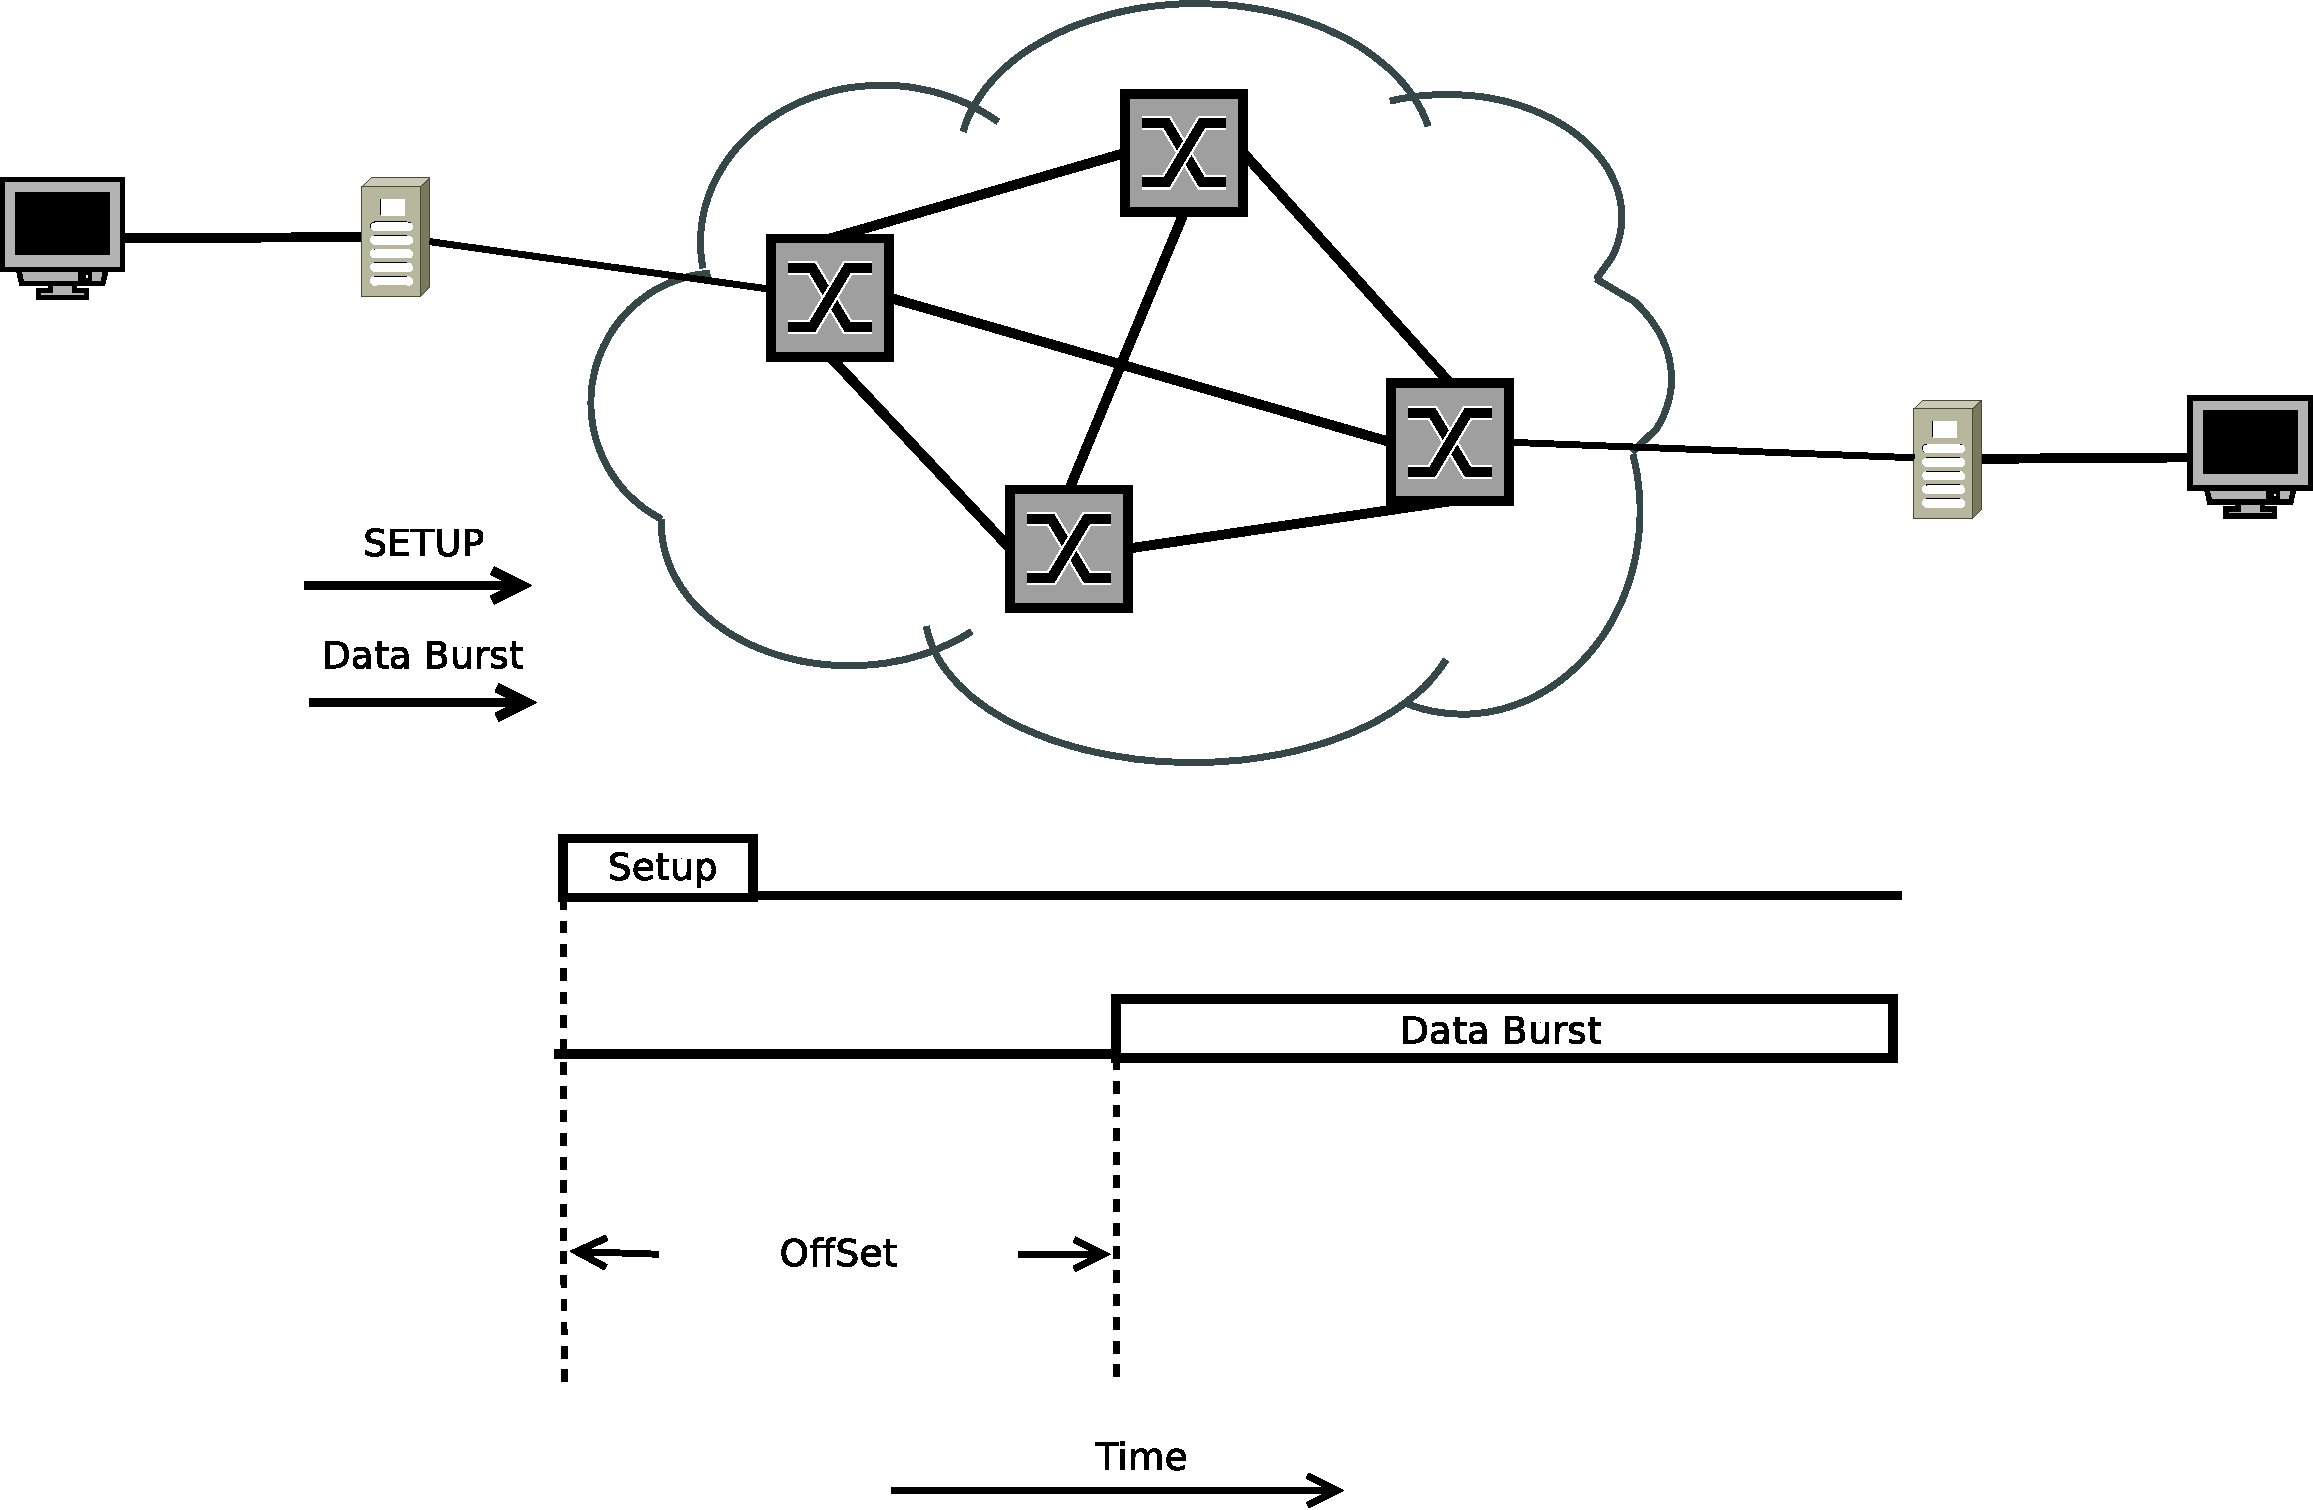
\includegraphics[height=6in]{setup}}
        \else
        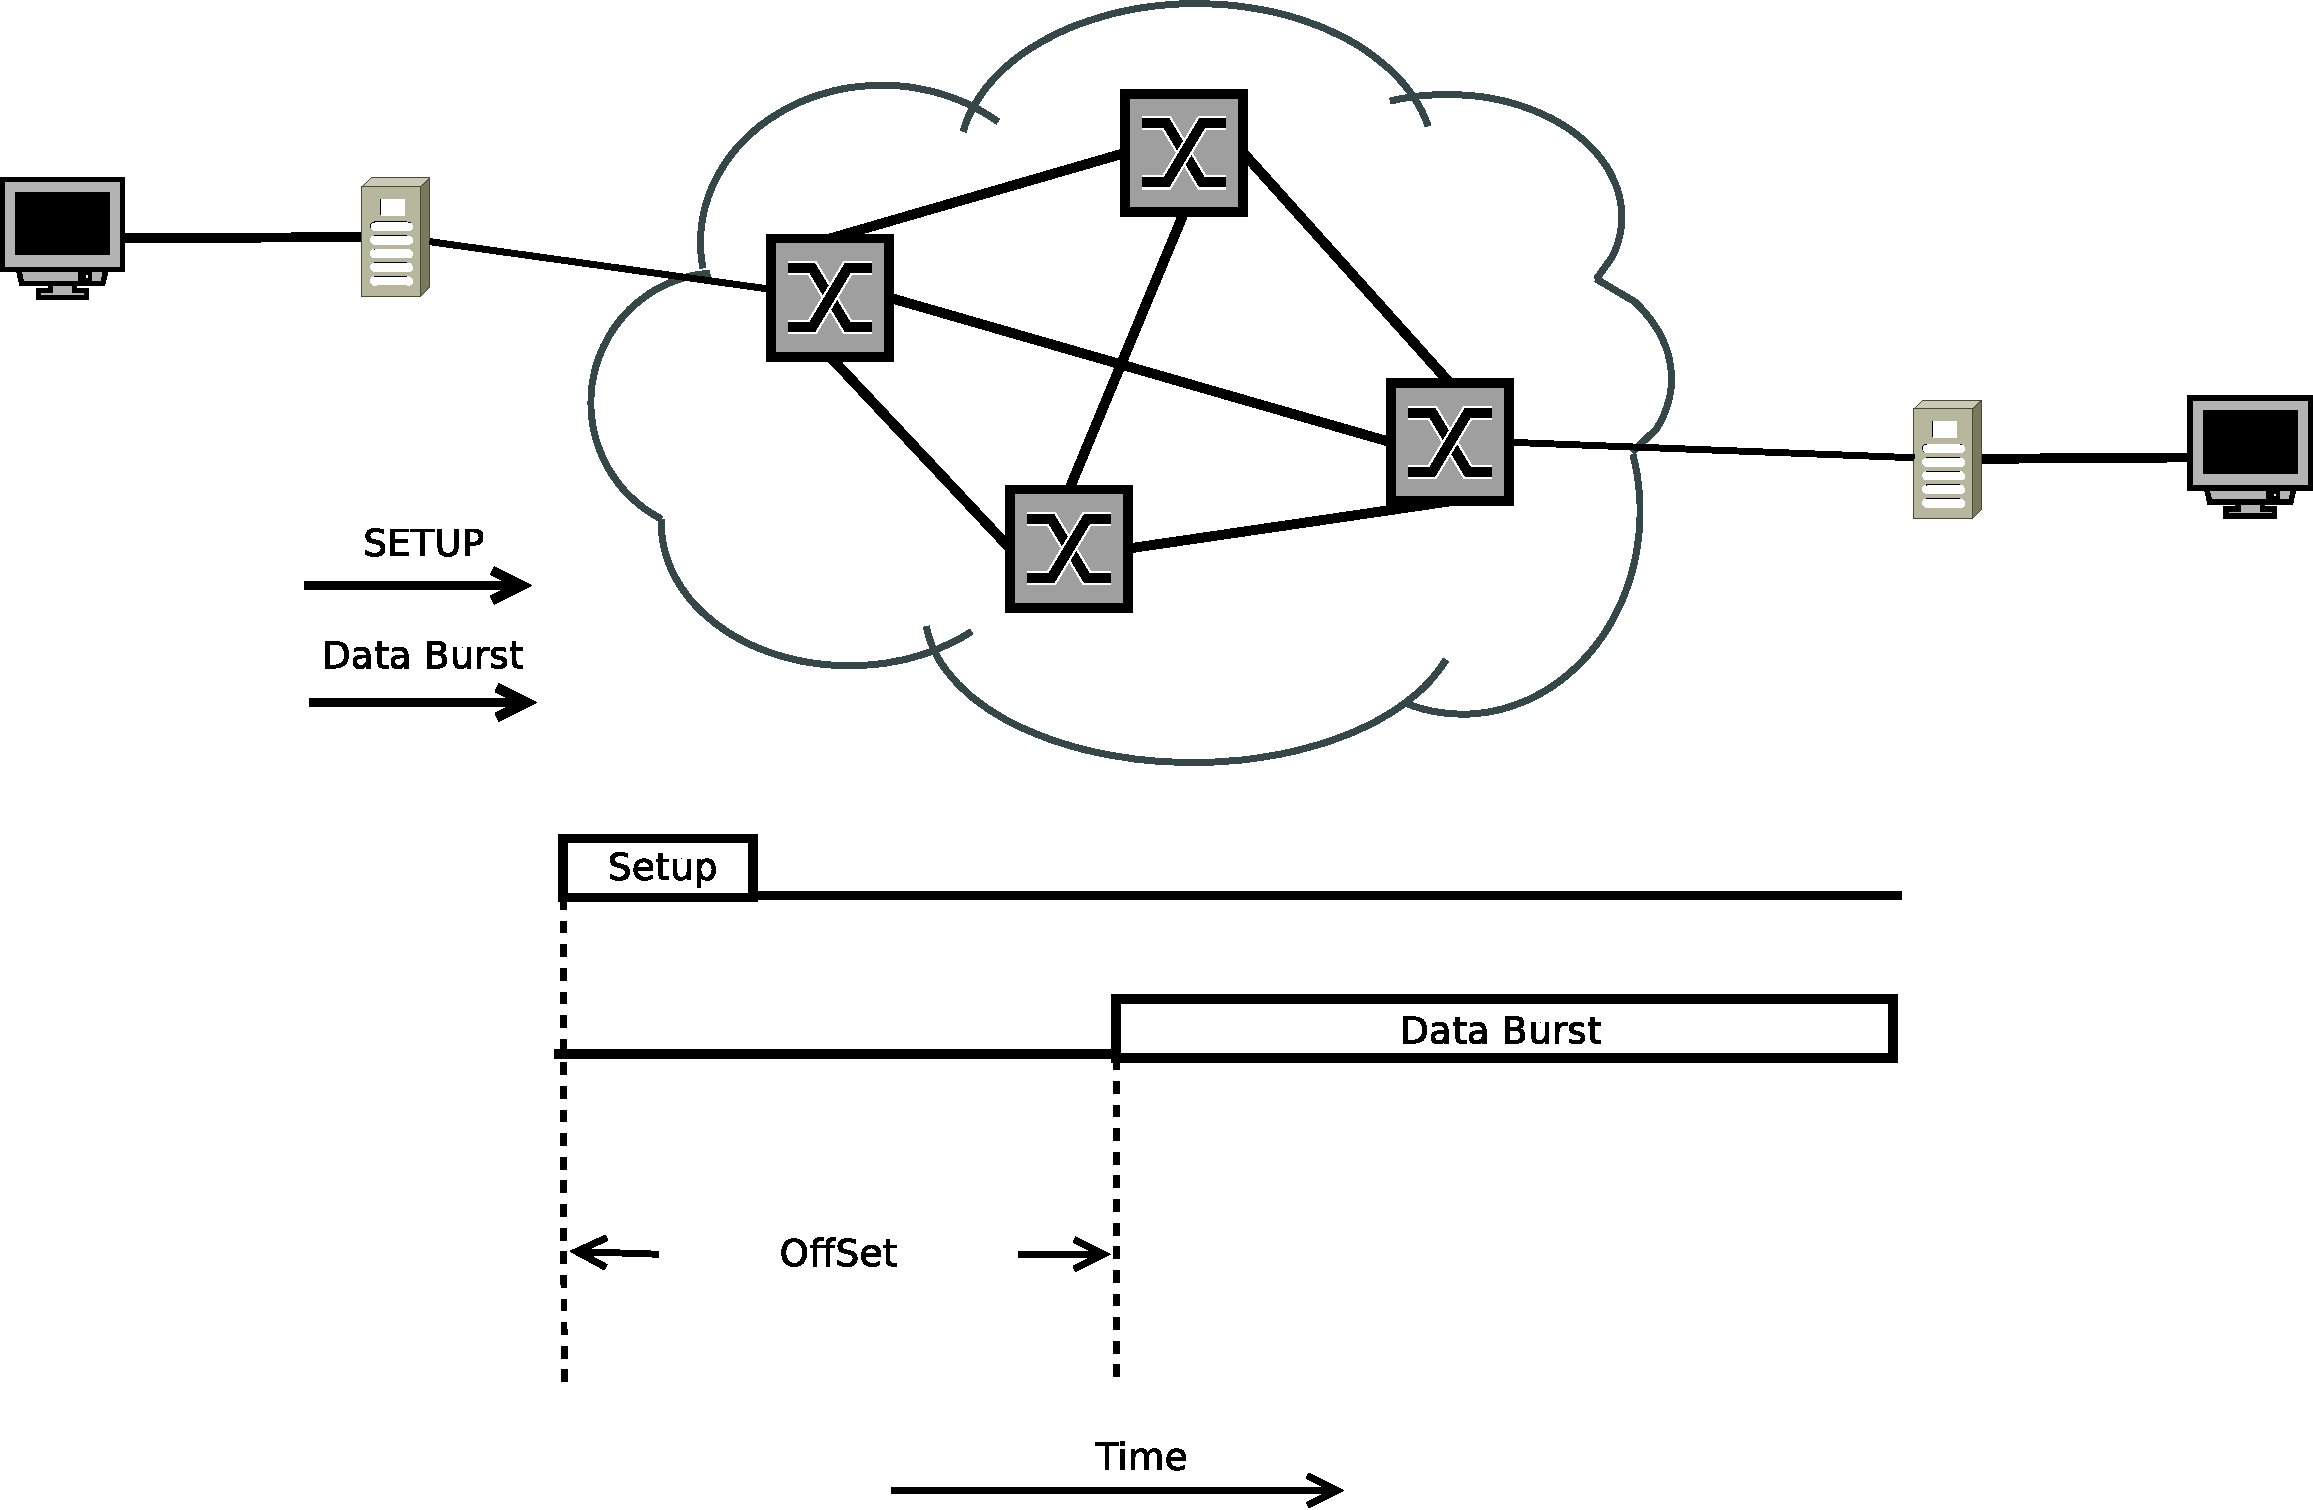
\includegraphics[bb = 92 86 545 742, height=6in]{setup}
        \fi
        \caption{Burst assembly,Burst reservation}
    \end{center}
\end{figure}

Among all optical switching technology, OBS seek to enhance the statistical multiplexing. It has proposed as a new paradigm switching technology for next generation Internet backbone network. Before we get closed to it. We need to get some foundational knowledge, such as what are the big characteristics of this form of exchange of technology. What is the biggest difference compare with traditional switching technology? Does it have born deficiency? 

\begin{figure}[!htb]
    \label{fig:obstime}
    \begin{center}
        \leavevmode
        \ifpdf
        \resizebox{120mm}{!}{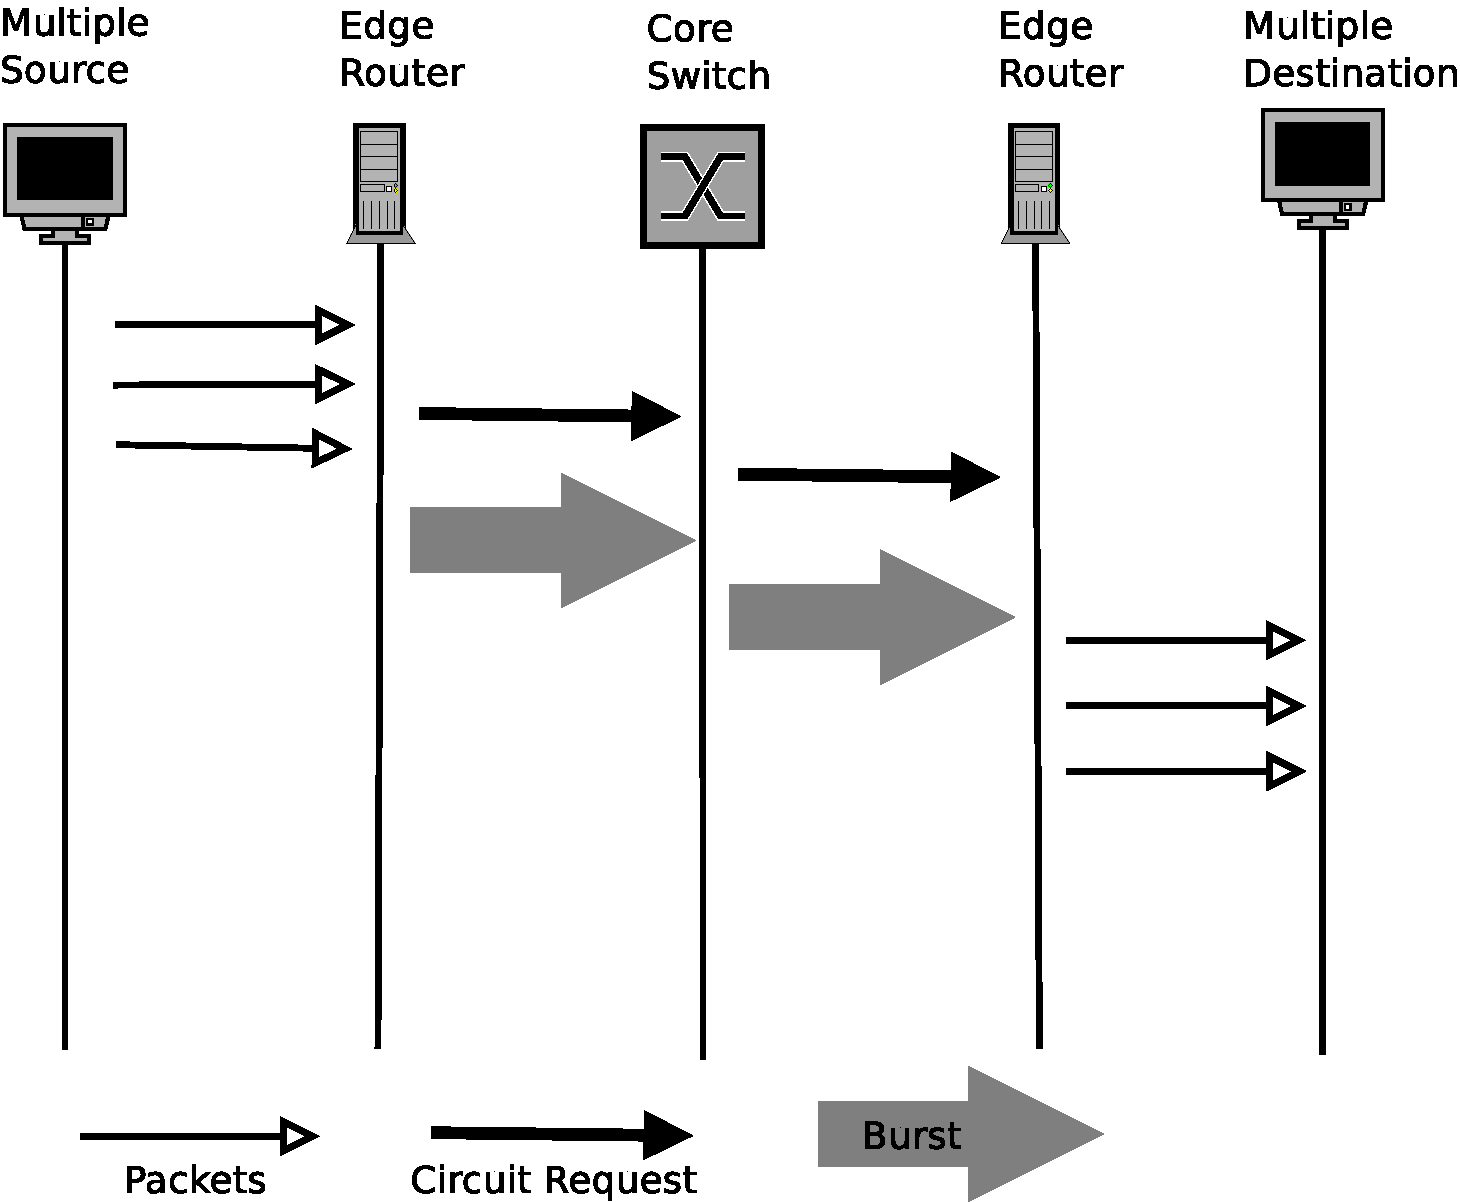
\includegraphics[height=6in]{burst}}
        \else
        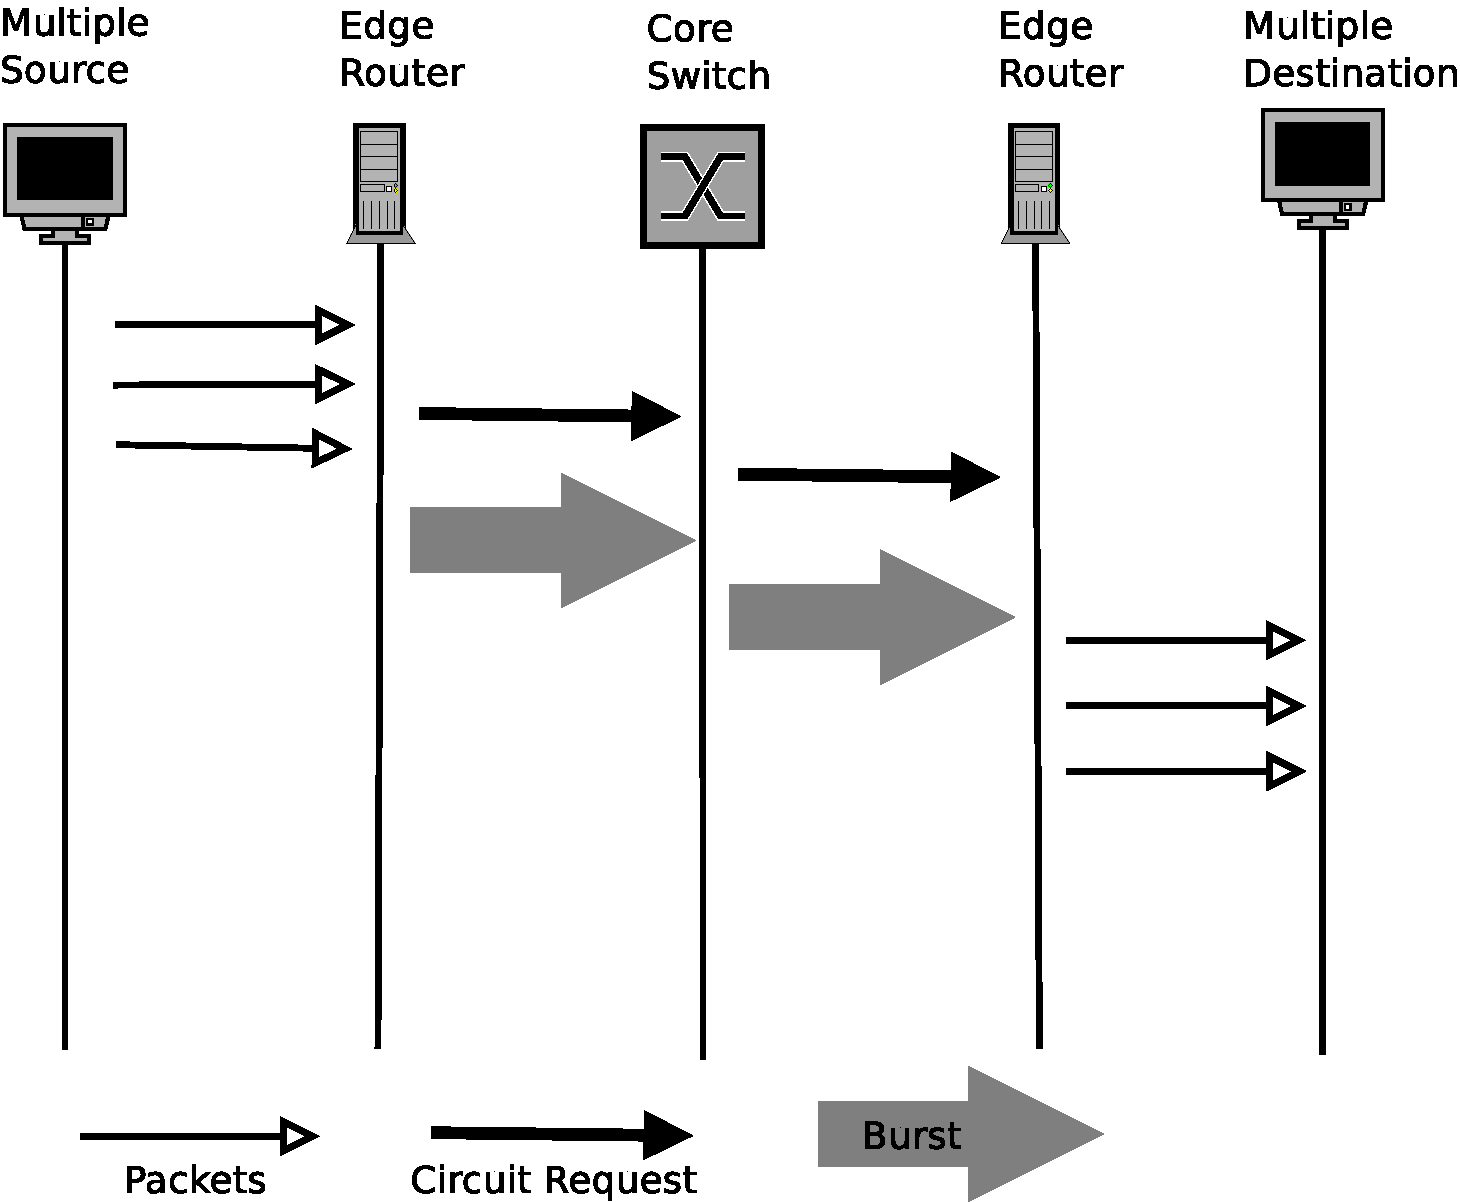
\includegraphics[bb = 92 86 545 742, height=6in]{burst}
        \fi
        \caption{Sample time diagram of a network using OBS}
    \end{center}
\end{figure}

\begin{figure}[!htb]
    \label{fig:burst_format}
    \begin{center}
        \leavevmode
        \ifpdf
        \resizebox{50mm}{!}{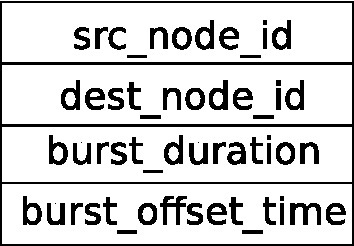
\includegraphics[height=6in]{burst_format}}
        \else
        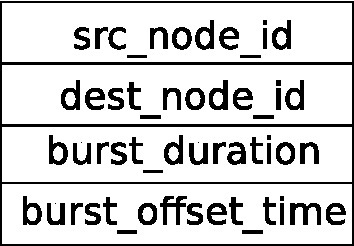
\includegraphics[bb = 92 86 545 742, height=6in]{burst_format}
        \fi
        \caption{OBS burst format sample}
    \end{center}
\end{figure}

The main different compare to conventional packet switching is bufferless on core node. OBS put all intelligent such as buffer, electronic processor, to edge side. As figure \ref{fig:obstransstep} show. All input data bursts are collected into bursts. There may be a classifier to classify packet to different burst according to their destination and Qos requirement or something else. After complete burst assemble and before the burst
transmission begins, a Burst Header Cell (BHC) is sent on the control channel that is separate from data burst channel, carry information about the destination of the burst, duration of the burst, the number of hops it pass through. A sample burst format is shown in figure \ref{fig:burst_format}

A burst switcher, once receiving the BHC, schedule and determine an outgoing link for leading toward the desired destination with an idle channel available, and
then establishes a connection between the channel specified in BHC and the channel through schedule algorithm by core switcher to transmit the burst. It also pass the BHC to next hops on the control channel of the selected link. After the core router prepare for arriving burst, the burst go through core router without additional operation. It also refer as one-way reservation. The burst just wait a certain offset time and don't need to check the ACK from reservation process. Once
burst arrive to core router, It can be transmit in whole optical domain. That is the reason why OBS better than others mechanism. The mechanism for resource reservation and release has been study for a long time. In simple term, There are four major combinations as table \ref{tab:setupclass} show.

\begin{table}[!htbp]
    \label{tab:setupclass}
    \centering
    \setlength{\extrarowheight}{1mm}
    \addtolength{\tabcolsep}{3mm}
    \begin{tabular}{|r|l|l|}
        \hline
        \backslashbox{release}{setup} & Immediate setup & Delay setup \\
        \hline
        \multirow{2}{*}{Immediate release} & Immediate setup & Delay setup\\
                                           & Immediate release & Immediate release\\
        \hline  
        \multirow{2}{*}{Explicit release} & Immediate setup& Delay setup \\
                                          & Explicit release & Explicit release \\
        \hline
    \end{tabular}
    \caption{Classification of reservation/release schemes}
\end{table}

There are two main scheduling mechanism, that is so called \verb|LAUC| and \verb|LAUC-VF|, \verb|LAUC| is abbreviation of First-Fit, Horizon, Latest Available Unscheduled Channel. And \verb|LAUC-VF| is abbreviation of \verb|LAUC| with Void Filling. Since \verb|LAUC-VF| is the improvement of \verb|LAUC|, I employ \verb|LAUC-VF| algorithm in simulation.

